\section{Finanzierungskonzepte von Browsern}\label{sec:finanzierungskonzepte-von-browsern}

\subsection{Rückblick}\label{subsec:rueckblick}
Schon im Jahr 2005, als Google gerade einmal 7 Jahre alt war,
kommentierte Prof.\ Dr.\ Jens Wolling die Finanzierung von Suchmaschinen mit
\("\)Eine Finanzierung [\ldots] allein aus Bannerwerbung ist unrealistisch\("\)\autocite{WOL05},
als weitere Finanzierungsquelle der privatwirtschaftlichen Großkonzerne führt er deshalb Verkauf von Technologie oder
Suchergebnissen an.\autocite{WOL05}\\

Den Trend zur damaligen Zeit analysiert er folgendermaßen: Es gäbe zwei mögliche Richtungen,
in die Finanzierung der Suchportale entwickeln könnte und es zum Teil auch schon tut.
Die erste Möglichkeit seien Aufnahmegebühren, in diesem Fall müssten Anbieter bezahlen,
um überhaupt erst von der Suchmaschine gefunden zu werden.
Die zweite Möglichkeit hingegen seien Platzierungsgebühren, wobei man für eine gute Platzierung bezahlen müsse.
Beide Varianten sieht Wolling durchaus kritisch.\autocite{WOL05}\\

Doch wie werden die großen Suchmaschinen und Mediengiganten heute finanziert?
Und wie finanzieren sich Start-ups und kleinere Unternehmen auf dem Markt?
Im Folgenden werden wichtigsten Finanzierungsmöglichkeiten analysiert.

\subsection{Finanzierung durch Werbung}\label{subsec:finanzierung-durch-werbung}
Werbung ist, wie wohl den meisten klar ist eines der größten Standbeine von Google und Co,
so hat Google, wie in der Statistik zu sehen, im Jahr 2021 einen Rekordumsatz von über 200 Milliarden US-Dollar durch Werbung umgesetzt,
mit einer stetig starken Steigerung des Umsatzes seit 2001.
Auch bei Bing und anderen großen Suchmaschinen sieht die Steigerung ähnlich aus, wenn auch in kleinerem Ausmaß.
\begin{figure}[ht]
    \centering
    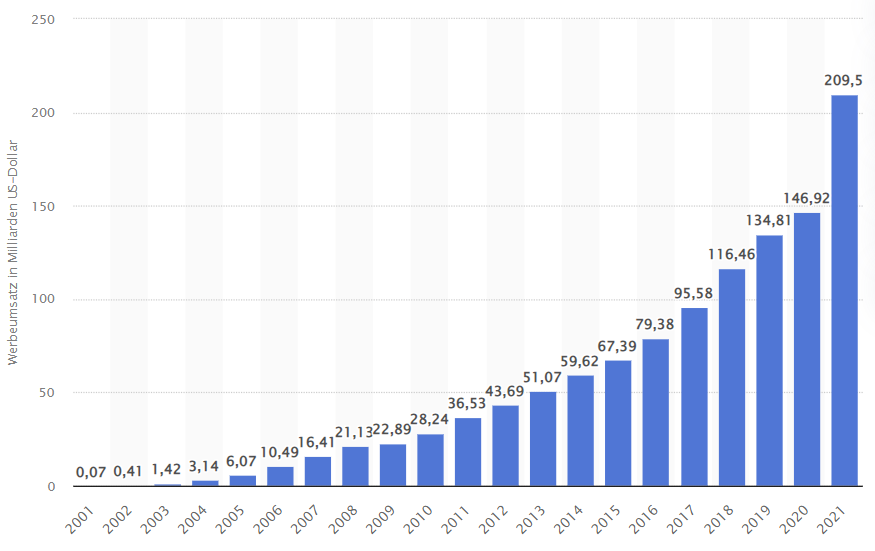
\includegraphics[width=100mm]{images/statistic_google_ads}
    \caption{Statistik Werbeumsätze Google in Milliarden}
    \label{fig:statisticAdsGoogle}
\end{figure}
Besonders in den letzten Jahren wurde auch personalisierte Werbung immer populärer.
Der Journalist und Author Dr. Björn Brückerhoff berichtet in einem Artikel 2020,
wie Google Daten aus nahezu allen Anwendungen, sowie der Suchmaschine selbst und Betriebssystemen,
wie in etwa Android, nutzt um Persönlichkeitsprofile seiner Nutzer zu erstellen.
Google kann laut Brückerhoff mithilfe dieser gigantischen Mengen an Daten auf \("\)Wünsche und Bedürfnisse,
die sexuelle Orientierung, die physische und psychische Gesundheit, die politischen Meinungen, die finanziellen Möglichkeiten,
die religiösen Überzeugungen oder die räumliche Flexibilität\("\)\autocite{BRK20} schließen.
Mithilfe dieser Persönlichkeitsdaten platziert Google dann die mithilfe von Algorithmen ermittelte,
am besten auf uns zugeschnittene Werbung.\autocite{BRK20}\\

Das Suchmaschinen-StartUp \("\)Qwant\("\) aus Frankreich gibt hingegen auf der Homepage der eigenen Suchmaschine nicht nur an,
keinerlei persönliche Daten zu verkaufen oder zu Werbezwecken zu nutzen, sondern auch diese persönlichen Daten nicht einmal zu erheben.
Die Suchmaschine finanziert sich laut Webseite \("\)kontextbasierte Werbung[, die] für alle gleich [ist]\("\)\autocite{QWA22},
jeder sieht also, unabhängig vorherigen Suchen, die gleiche Werbung.

Bei Ergebnissen zu Suchanfragen kann bei den meisten Suchmaschinen, so auch bei Google,
Bing und Qwant zwischen \("\)Anzeigen\("\) und \("\)organischen Treffern\("\) unterschieden werden.
Anzeigen, auch unter dem Begriff \("\)Paid Listings\("\) bekannt, bezeichnen bezahlte Suchtreffer,
die von Suchmaschinen in die Suchergebnisse \("\)gemischt\("\) werden.
Solche Anzeigen müssen nach EU-Recht als solche gekennzeichnet werden.\\
Organische Treffer sind hingegen Treffer, die durch Algorithmen der Suchmaschine als am besten passend auf die aktuelle Suche bewertet werden.
In der folgenden Statistik wird die Anzahl der als \("\)Anzeige\("\) gekennzeichneten Treffern unter den ersten zehn Treffern auf ausgewählten Suchanfragen gezeigt.\autocite{LEW18}\\
\begin{figure}[ht]
    \centering
    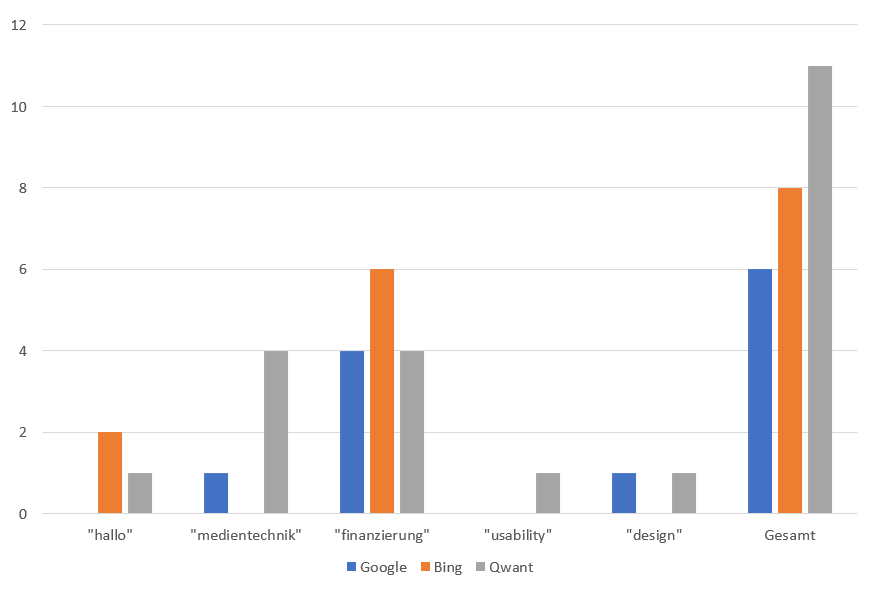
\includegraphics[width=100mm]{images/statistic_adverts}
    \caption{Statistik Anzeigen unter den ersten zehn Treffern bei ausgewählten Suchanfragen}
    \label{fig:statisticAdverts}
\end{figure}
Auffallend ist, dass Qwant insgesamt die meisten Anzeigen platziert hat, was allerdings daraus resultieren könnte,
dass es angibt keine Cookies wie Google und Bing zu verwenden, weshalb eine signifikante Einnahmequelle der Konkurrenz bei Qwant ausfällt.
Schaut man sich die Platzierungen der Anzeigen an, so fällt auf, dass Qwant diese oft,
im Gegensatz zu Bing und Google am Ende der aufgezeigten Suchergebnisse zeigt.
Auch fällt auf, dass der Anbieter mit den meisten Anzeigen bei fast jeder Anzeige sehr unterschiedlich ausfällt,
weshalb das Ergebnis auch stark von den gewählten Suchbegriffen abhängen könnte.\\